\documentclass[12pt]{article}
\usepackage[margin=2.5cm]{geometry}
\usepackage{enumerate}
\usepackage{amsfonts}
\usepackage{amsmath}
\usepackage{fancyhdr}
\usepackage{amsmath}
\usepackage{amssymb}
\usepackage{amsthm}
\usepackage{mdframed}
\usepackage{graphicx}
\usepackage{subcaption}
\usepackage{adjustbox}
\usepackage{listings}
\usepackage{xcolor}
\usepackage{booktabs}
\usepackage[utf]{kotex}
\usepackage{hyperref}

\definecolor{codegreen}{rgb}{0,0.6,0}
\definecolor{codegray}{rgb}{0.5,0.5,0.5}
\definecolor{codepurple}{rgb}{0.58,0,0.82}
\definecolor{backcolour}{rgb}{0.95,0.95,0.92}

\lstdefinestyle{mystyle}{
    backgroundcolor=\color{backcolour},
    commentstyle=\color{codegreen},
    keywordstyle=\color{magenta},
    numberstyle=\tiny\color{codegray},
    stringstyle=\color{codepurple},
    basicstyle=\ttfamily\footnotesize,
    breakatwhitespace=false,
    breaklines=true,
    captionpos=b,
    keepspaces=true,
    numbers=left,
    numbersep=5pt,
    showspaces=false,
    showstringspaces=false,
    showtabs=false,
    tabsize=1
}

\lstset{style=mystyle}

\pagestyle{fancy}
\renewcommand{\headrulewidth}{0.4pt}
\lhead{Team Treehouse}
\rhead{Regular Expressions in Java Notes}

\begin{document}
\title{Regular Expressions in Java Notes}
\author{Team Treehouse}
\maketitle

\begin{itemize}
    \item Resources
    \begin{itemize}
        \item \textbf{Java Pattern Documentation:} \href{https://docs.oracle.com/javase/8/docs/api/java/util/regex/Pattern.html}{link}
        \item \textbf{Online Java Regex tester:} \href{https://www.freeformatter.com/java-regex-tester.html}{link}
    \end{itemize}
    \item \textit{STRING\_VAR.matches(...)}
    \begin{itemize}
        \item Tells if the string matches the given regular expression
        \item Is equivalent to `\textit{\^REGEX\_EXPRESSION\$}'
        \item Can be used to validate something

        \bigskip

        \underline{\textbf{Example:}}

        \bigskip

    \begin{lstlisting}[language=Java, caption={demo/Explore1.java}]
    Console console = System.console();
    String zipCode = "90210";
    if (zipCode.matches("^\\d{5}(-\\d{4})?$")) {
    System.out.printf("%s is a valid zip code%n", zipCode);
    } else {
    System.out.printf("%s is NOT a valid zip code%n", zipCode);
    }

    // Returns '90210 is a valid zip code'
    \end{lstlisting}

    \end{itemize}

    \item \textit{STRING\_VAR.split(...)}
    \begin{itemize}
        \item Splits string by the regex pattern
        \item $\backslash$ W+ means NOT words
        \item (...)? means optional, i.e. can be included, but it's okay if its
        not included

        \begin{center}
        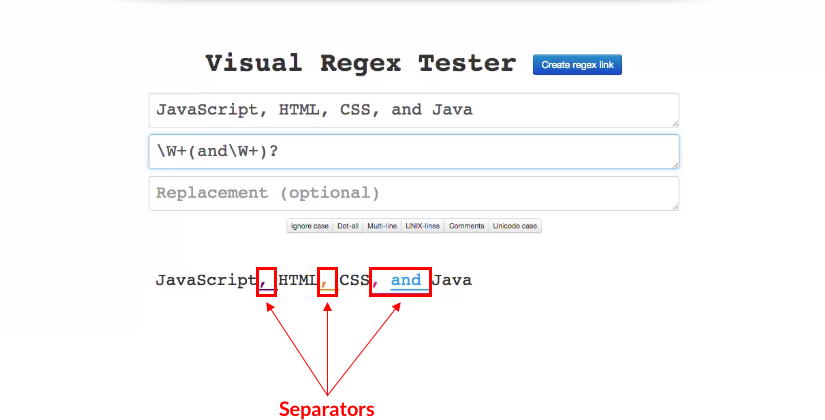
\includegraphics[width=\linewidth]{images/image_1.png}
        \end{center}

        \bigskip

        \underline{\textbf{Example:}}

        \bigskip

    \begin{lstlisting}[language=Java, caption={demo/Explore2.java}]
    String skills = "JavaScript, HTML, CSS, and Java";
    for (String skill : skills.split("\\W+(and\\W+)?")) {
        System.out.printf("Skill : %s \n", skill);
    }

    // Returns
    // Skill : JavaScript
    // Skill : HTML
    // Skill : CSS
    // Skill : Java
    \end{lstlisting}

    \end{itemize}

    \item

    \textit{Pattern pattern = Pattern.compile(REGEX\_PATTERN);}

    \textit{Matcher matcher = pattern.matcher(STRING\_VAR)}

    \begin{itemize}
        \item Returns all words matching pattern
        \item Note: (...) means a group
    \end{itemize}

    \begin{center}
    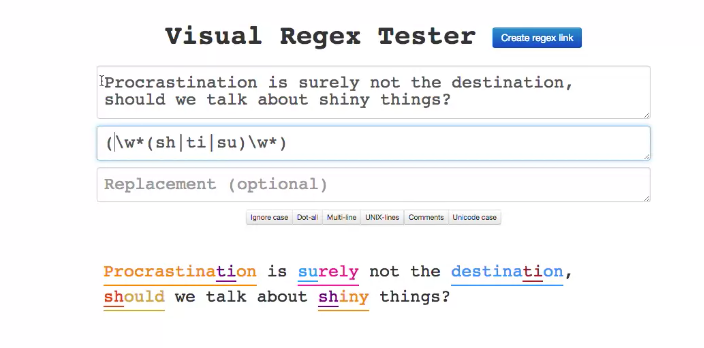
\includegraphics[width=\linewidth]{images/image_2.png}
    \end{center}


    \bigskip

    \underline{\textbf{Example:}}

    \bigskip

    \begin{lstlisting}[language=Java, caption={demo/Explore3.java}]
    String script = "Procrastination is surely not the destination, should we talk about shiny things?";

    Pattern pattern = Pattern.compile("(\\w*(sh|ti|su)\\w*)",
                                        Pattern.CASE_INSENSITIVE);
    Matcher matcher = pattern.matcher(script);

    while (matcher.find()) {
        System.out.printf("%s is a shushy word because of %s \n",
                            matcher.group(1), // <- returns value of outer parenthesis
                            matcher.group(2)); // <- returns value of inner parenthesis
    }

    // Returns
    // Procrastination is a shushy word because of ti
    // surely is a shushy word because of su
    // destination is a shushy word because of ti
    // should is a shushy word because of sh
    // shiny is a shushy word because of sh
    \end{lstlisting}

\end{itemize}

\end{document}